\chapter{Verbreitung von \acl{2FA}}

Die Nutzungsraten von \ac{2FA} sind weiterhin gering. Laut \textcite{petsasTwofactorAuthentication2015} wenden nur 6,4\% der Nutzerinnen die Zwei-Schritt-Verifizierung von Google an, während diese Rate bei anderen Anbietern nur 2-5\% betrage. Im professionellen Bereich wurden hingegen sogar 17\% festgestellt \parencite{ackermanImpedimentsAdoption2020}. Abbildung \ref{fig:motivation} zeigt jedoch, dass in professionellen Kontexten \ac{2FA} oft nicht aus eigenem Antrieb, sondern aus Pflicht genutzt werden \parencite{decristofaroComparativeUsability2014}. Da im Privaten eine \ac{2FA}-Pflicht schwieriger durchzusetzen ist, insbesondere ohne die Nutzerinnen zu vergraulen, gilt es herauszufinden, was sie davon abhält und wie sie zur Nutzung von \ac{2FA} gebracht werden können.

\begin{figure}
  \begin{center}
    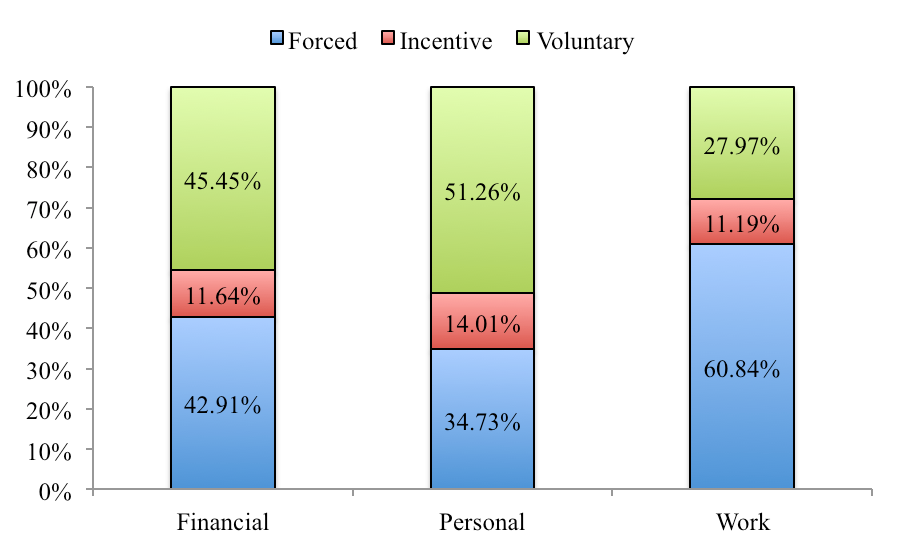
\includegraphics[width=0.95\textwidth]{assets/motivation.png}
  \end{center}
  \caption[Motivation für die Nutzung von \acs{2FA} in verschiedenen Kontexten]{Motivation für die Nutzung von \acs{2FA} in verschiedenen Kontexten.\\\parencite[6]{decristofaroComparativeUsability2014}}
  \label{fig:motivation}
\end{figure}

% \parencite{gargHeuristicsBiases2013} (7 in \textcite{dasWhyJohnny2018})

\textcite{dasWhyJohnny2018} nennen ein mangelndes Bewusstsein für Sicherheitsrisiken und die daraus entstehende Wahrnehmung, dass die Verwendung von \ac{2FA} keinen Mehrwert hat, als primären Grund für die mangelnde Akzeptanz von \ac{2FA}. In der Studie von \parencite{ackermanImpedimentsAdoption2020} wurde ein ähnliche Meinung als zweithäufigster Grund\footnote{Am häufigsten wurde fehlende Zeit als Grund genannt. Abgesehen von Möglichkeiten, den Einrichtungsprozess zu optimieren und darüber zu informieren, soll hier jedoch der Augenmerk auf inhaltlichen Gründen liegen.} genannt, \ac{2FA} nicht einzurichten. Die Teilnehmerinnen glaubten nicht, dass ihre Accounts Ziel von Cyberattacken werden könnten \parencite{ackermanImpedimentsAdoption2020}. Um Nutzerinnen zu überzeugen, \ac{2FA} zu nutzen, hilft es, sie darüber aufzuklären. Dazu ist eine Nachricht, welches Risiken auf einem persönlichen Level aufdeckt, eine Gegenmaßnahme (Nutzung von \ac{2FA}) vorschlägt und zeigt, wie einfach die Umsetzung dieser ist, geeignet \parencite{ackermanImpedimentsAdoption2020}.

Zu beachten ist jedoch, dass laut \textcite{ackermanImpedimentsAdoption2020} eine erhöhte Wahrnehmung des Stärkegrades der Risiken nicht zu einer höheren Einführungsrate von \ac{2FA} führte. Die Nutzerinnen reagieren also nicht in einem verstärkten Maße auf drohende Nachrichten \parencite{ackermanImpedimentsAdoption2020}.

Abgesehen von den Risiken der Nichtnutzung sollten auch die Vorteile der Nutzung von \ac{2FA} kommuniziert werden, da Menschen Entscheidungen treffen, indem sie Vorteile und Risiken miteinander abwägen \parencite{dasWhyJohnny2018}. Dieser Theorie folgend sollten Sicherheitssystem konstruiert werden, um die Verbreitung zu verbessern \parencite{gargHeuristicsBiases2013}.

\pskip
In der Studie von \textcite{dasWhyJohnny2018} wurde mehrfach geäußert, dass die Teilnehmerinnen bereits vollstes Vertrauen in ihre Sicherheitsvorkehrungen und Passwortwahl hatten. Damit einher ging ein Missverständnis über die Funktionsweise von \ac{2FA}, welcher von \textcite{ackermanImpedimentsAdoption2020} als dritthäufigster Grund genannt wurde, \ac{2FA} nicht einzurichten. Klare Kommunikation kann Unsicherheiten über den Einrichtungsprozess, die Funktionsweise und die Zuverlässigkeit von \ac{2FA} beseitigen \parencite{ackermanImpedimentsAdoption2020}.

Damit einher geht eine Gruppe von Nutzerinnen, denen Vertrauen in die eigene Fähigkeit, \ac{2FA} einzurichten und zu nutzen, fehlt \parencite{ackermanImpedimentsAdoption2020}. \textcite{ackermanImpedimentsAdoption2020} betont, dass dieses Selbstvertrauen benötigt wird, um Nutzerinnen dazu zu bewegen, \ac{2FA} zu nutzen.

\pskip
\textcite{dasWhyJohnny2018} schlagen vor, die Vorteile der Nutzung von \ac{2FA} für Nutzerinnen zu vergrößern, um so Anreize zur Nutzung von \ac{2FA} zu schaffen. Der erfahrene Wert von \ac{2FA} wird dadurch gesenkt, dass weiterhin das Passwort ausgedacht, gemerkt und eingegeben werden muss \parencite{dasWhyJohnny2018}. Es wird vorgeschlagen, die Authentifizierung zu vereinfachen, wenn \ac{2FA}-Mittel genutzt werden: Es könnte beispielsweise nicht nach dem vollen Passwort gefragt werden, falls \ac{2FA} auf einem bekannten Gerät genutzt wird \parencite{dasWhyJohnny2018}.

\pskip
\textcite{colnagoItsNot2018} stellen die Wichtigkeit einer guten Implementierung von \ac{2FA} hervor. Dabei sollte sowohl auf die Einrichtung, als auch auf die alltägliche Nutzung geachtet werden, um eine Verärgerung von Nutzerinnen zu verhindern \parencite{colnagoItsNot2018}. Eine gute Implementierung achtet darauf, die Nutzerinnen zu unterstützen und weniger negative Situationen zu schaffen \parencite{colnagoItsNot2018}.

In institutionellen Kontexten stellen \ac{2FA}-Pflichten ein valides Mittel dar, um Nutzungsraten zu verbessern. Während bei einer Durchsetzung durch Pflicht mehr negative Erfahrungen aufgezeichnet wurden, sagten die Nutzerinnen auch aus, dass es einfacher als erwartet war \parencite{colnagoItsNot2018}. Vielleicht können solche Erfahrungen auch das Nutzungsverhalten bei privaten Anwendungen beeinflussen.
